

\documentclass[12pt]{extarticle}

\usepackage{summary-intro}



\begin{document}



\sumintro{Non-Measurable Sets}{Spring 2023}



\section{Additive notions of size}


\begin{itemize}

\item the \textbf{length} of two (non-overlapping) line segments placed side by side is the length of the first plus the length of the second; 

\item the \textbf{mass} of two (non-overlapping) objects taken together is the mass of the first plus the mass of the second. 

\item the \textbf{probability} that either of two (incompatible) events occur is the probability that the first occurs plus the probability that the second occurs; 

\end{itemize}
The notion of \textbf{measure} is a very abstract way of thinking about additive notions of size.


\section{Generalizing the notion of length}


The standard notion of length:
\begin{itemize}
\item $[a,b] = \set{x \in \mathbb{R} : a \leq x \leq b}$

\item Length$\left([a,b]\right) = b - a$.
\end{itemize}



\subsection{The Borel Sets}
\label{sec:borel-sets}

A \textbf{Borel Set} is a set that you can get to by performing finitely many applications of the operations of \emph{complementation} and \emph{countable union} on a family of line segments.\footnote{Formally, the Borel Sets are the members of the smallest set $\mathscr{B}$ such that: $(i)$ every line segment is in $\mathscr{B}$, $(ii)$ if a set is in $\mathscr{B}$, then so is its complement, and $(iii)$ if a countable family of sets is in $\mathscr{B}$, then so is its union.}


\begin{itemize}
\item The \textbf{complementation operation} takes each set $A$ to its complement, $\overline{A}= \mathbb{R}-A$.


\item The \textbf{countable union operation} takes each countable family of sets $A_1, A_2, A_3, \ldots$ to their union, $\bigcup \{A_1, A_2 , A_3 \dots\}$.\label{gloss:count-un} 



\end{itemize}




\subsection{Lebesgue Measure}

There is exactly one function $\lambda$ on the Borel Sets that satisfies these three conditions:\label{gloss:leb-measurable}
\begin{description}
\item[Length on Segments] $\lambda([a,b]) = b-a$ for every $a,b \in \mathbb{R}$.\label{gloss:lls}



\item[Countable Additivity]
\[\lambda\left(\bigcup\{A_1,  A_2 , A_3,\ldots\}\right) = \lambda(A_1) + \lambda(A_2) + \lambda(A_3) + \ldots\] whenever $A_1,A_2,\dots$ is a countable family of disjoint sets for each of which $\lambda$ is defined.\label{gloss:count-add-measure}



\item[Non-Negativity]
$\lambda(A)$ is either a non-negative real number or the infinite value $\infty$, for any set $A$ in the domain of $\lambda$.\label{gloss:non-neg}



 \end{description}
 
 \begin{itemize}
 

\item a function on the Borel Sets is a \textbf{measure} if and only if it satisfies Countable Additivity and Non-Negativity (and assigns the value 0 to the empty set).\label{gloss:measure} 


 \item the \textbf{Lebesgue Measure} is the (unique) measure $\lambda$ that satisfies Length on Segments.\footnote{We say that a set  $A \subseteq \mathbb{R}$ is \textbf{Lebesgue Measurable} if and only if $A = A^B \cup A^0$, for $A^B$  a Borel Set and $A^0$ a subset of some Borel Set of Lebesgue Measure zero.  We apply $\lambda$ to Lebesgue measurable sets that are not Borel sets by stipulating that  $\lambda(A^B \cup A^0) = \lambda(A^B)$. }
 
 \end{itemize}



\section{Uniformity}
\label{sec:uniformity}

The Lebesgue Measure, $\lambda$, satisfies:
\begin{description}
\item[Uniformity]
$\mu(A^c) = \mu(A)$, whenever $\mu(A)$ is well-defined and $A^c$ is the result of adding $c \in \mathbb{R}$ to each member of $A$.\label{gloss:uniformity}
\end{description}





\subsection{Probability Measures}
\label{sec:coin-toss-procedures}





Two ways of randomly selecting a number from $[0,1]$:
\begin{description}


\item[Standard Coin-Toss Procedure]
You toss a fair coin once for each natural number. Each time the coin lands Heads you write down a zero, and each time it lands Tails you write down a one. This gives you an infinite binary sequence $\langle d_1,d_2,d_3,\ldots\rangle$, Pick $0.d_1d_2d_3\ldots$ (in binary notation).\footnote{Rational numbers have two different binary expansions: one ending in 0s and the other ending in 1s. To simplify the present discussion, I assume that the Coin-Toss Procedure is rerun if the output corresponds to a binary expansion ending in 1s.}

\begin{itemize}
\item We get uniformity:
\vspace{7mm}
\begin{center}
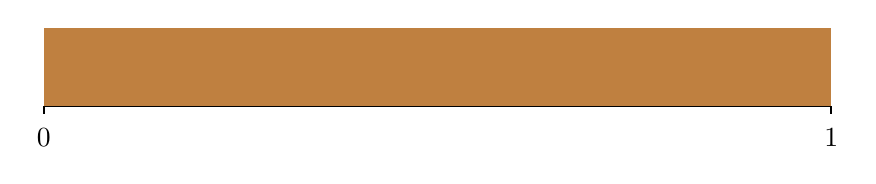
\begin{tikzpicture}
\fill[brown] (5cm,0cm) rectangle (-5cm,1cm); %mud
\draw[line width=0.02cm] (-5,0) -- (5,0); % x axis
\draw[line width=0.02cm] (-5,0) -- (-5,-0.1); % 0 tick
\node at (-5,-0.4) {0}; % 0 label
\draw[line width=0.02cm] (5,0) -- (5,-0.1); % 1 tick
\node at (5,-0.4) {1}; % 1 label
\end{tikzpicture}
\end{center}
\item Given certain assumptions about the probabilities of sequences of coin tosses, we get the Lebesgue Measure.


\end{itemize}


\item[Square Root Coin-Toss Procedure]
As before, but this time you pick $\sqrt{0.d_1d_2d_3\ldots}$ (in binary notation). 

\begin{itemize}

\item We do not get uniformity:



\vspace{7mm}
\begin{center}
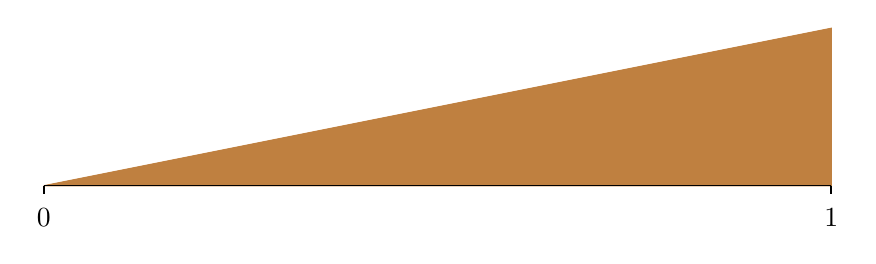
\begin{tikzpicture}
\draw [draw=brown, fill=brown] (-5,0) -- (5,0) -- (5,2) -- cycle; %mud
\draw[line width=0.02cm] (-5,0) -- (5,0); % x axis
\draw[line width=0.02cm] (-5,0) -- (-5,-0.1); % 0 tick
\node at (-5,-0.4) {0}; % 0 label
\draw[line width=0.02cm] (5,0) -- (5,-0.1); % 1 tick
\node at (5,-0.4) {1}; % 1 label

\end{tikzpicture}
\end{center}

\end{itemize}

\end{description}




\section{Non-Measurable Sets}
\label{sec:non-measurable-sets}


\begin{itemize}
\item There are subsets of $\mathbb{R}$ that are \textbf{non-measurable}:

They cannot be assigned a measure by any {extension} of $\lambda$, without giving up on Non-Negativity, Countable Additivity, or Uniformity.

\end{itemize}




\section{The Axiom of Choice}\label{the-axiom-of-choice}

Proving that there are non-measurable sets requires:

\begin{description}
\item[Axiom of Choice]
Every set of non-empty, non-overlapping sets has a choice set.
\end{description}
(A \textbf{choice set} for set $A$ is a set that contains exactly one member from each member of $A$.)



\section{Defining the Vitali Sets}

\subsection{A sketch of the construction}

\begin{itemize}

\item Define an (uncountable) partition $\mathcal{U}$ of $[0,1)$.

\item Use the Axiom of Choice to pick a representative from each cell of $\mathcal{U}$.

\item Use these representatives to define a (countable) partition $\mathcal{C}$ of $[0,1)$.

\item A Vitali Set is a cell of $\mathcal{C}$.

\end{itemize}


\subsection{Defining $\mathcal{U}$}

\begin{quote}

 $a, b \in [0,1)$ are in the same cell if and only if $a - b \in \mathbb{Q}$.


\end{quote}




\subsection{Defining $\mathcal{C}$}


\begin{itemize}
\item $\mathcal{C}$ has a cell $C_q$ for each rational number $q \in \mathbb{Q}^{[0,1)}$.

\item $C_0$ is the set of representatives of cells of $\mathcal{U}$.

\item $C_q$ is the set of numbers $x \in [0,1)$ which are at a ``distance'' of $q$ from the representative of their cell in $\mathcal{U}$.
\end{itemize}
Here ``distance'' is measured by bending $[0,1)$ into a circle:
\vspace{3mm}
\begin{center}
\begin{tikzpicture}[scale = 0.75]
\draw[thin] (-10,0) -- (-5.03,0); % straight line axis
\draw[very thin] (-10,0) -- (-10,-0.1); % 0 tick on straight
\node at (-10,-0.4) {\tiny 0}; % 0 label on straight
%\draw[very thin] (-5,-.03) -- (-5,-0.1); % 1 tick on straight
\draw (-5,0) circle [radius=0.03]; %circle at 1
\node at (-5,-0.4) {\tiny 1}; % 1 label on straight
\draw (0,0) circle [radius=0.795774715cm]; %circle
\draw[very thin] (90:0.795774715cm) -- (90:0.895774715cm); % 0 tick on circle
\node at (0,1.1) {\tiny 0 1}; % 0 label on circle
\draw[very thick, ->] (-3.6,0) -- (-2.1,0); %arrow
\end{tikzpicture}
\end{center}
and traveling counter-clockwise. For instance, $\frac{1}{4}$ is at ``distance'' $\frac{1}{2}$ from $\frac{3}{4}$:
\vspace{5mm}
\begin{center}
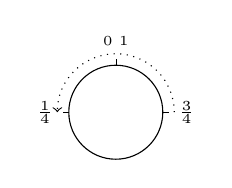
\begin{tikzpicture}[scale = 0.75]
\draw (0,0) circle [radius=0.795774715cm]; %circle
\draw[very thin] (90:0.795774715cm) -- (90:0.895774715cm); % 0 tick on circle
\node at (0,1.2) {\tiny 0 1}; % 0 label on circle
\draw[very thin] (0:0.795774715cm) -- (0:0.895774715cm); % 3/4 tick on circle
\node at (1.2,0) {\tiny $\frac{3}{4}$}; % 3/4 label on circle
\draw[->, dotted] (0.99cm,0) arc [start angle = 0, end angle = 180, radius=0.99cm]; %big circle
\draw[very thin] (180:0.795774715cm) -- (180:0.895774715cm); % 1/4 tick on circle
\node at (-1.2,0) {\tiny $\frac{1}{4}$}; % 1/4 label on circle
\end{tikzpicture}
\end{center}



\section{A Vitali Set Cannot Be Measured}

\subsection{Assumptions}

\begin{description}


\item[Countable Additivity]
\[\lambda\left(\bigcup\{A_1,  A_2 , A_3,\ldots\}\right) = \lambda(A_1) + \lambda(A_2) + \lambda(A_3) + \ldots\] whenever $A_1,A_2,\dots$ is a countable family of disjoint sets for each of which $\lambda$ is defined.\label{gloss:count-add-measure}



\item[Non-Negativity]
$\lambda(A)$ is either a non-negative real number or the infinite value $\infty$, for any set $A$ in the domain of $\lambda$.\label{gloss:non-neg}


\item[Uniformity]
$\mu(A^c) = \mu(A)$, whenever $\mu(A)$ is well-defined and $A^c$ is the result of adding $c \in \mathbb{R}$ to each member of $A$.\label{gloss:uniformity}
\end{description}

\subsection{The Proof}

\begin{itemize}
\item Suppose otherwise: $\lambda(C_q)$  is well-defined for some $q \in \mathbb{Q}^{[0,1)}$.  

\item By Uniformity, $\lambda(C_q') = \lambda(C_q)$ for any $q' \in \mathbb{Q}^{[0,1)}$.

\item By Non-Negativity, $\lambda(C_q)$ is either $0$, or a positive real number, or $\infty$.

\item By Countable Additivity, it can't be any of these:



\begin{itemize}
\item Suppose $\lambda(C_q) =0$. By Countable Additivity:
\[
\begin{array}{ccc}
\lambda([0,1)) &= &\lambda(C_q) + \lambda(C_{q'}) + \ldots\\
&= &\parbox{30mm}{\vspace{3mm}$\underbrace{0 + 0 + 0 + \ldots}_{\text{\tiny once for each integer}}$} \\
&= &\parbox{30mm}{\vspace{3mm}$0$}
\end{array}
\]


\item Suppose $\lambda(C_q) = r >0$. By Countable Additivity:
\[
\begin{array}{ccc}
\lambda([0,1)) &= &\lambda(C_q) + \lambda(C_{q'}) + \ldots\\
&= &\parbox{30mm}{\vspace{3mm}$\underbrace{r + r + r + \ldots}_{\text{\tiny once for each integer}}$} \\
&= &\parbox{30mm}{\vspace{3mm}$\infty$}
\end{array}
\]


\end{itemize}



\end{itemize}
\emph{Moral:} There is no way of assigning a measure to a Vitali set without giving up on Uniformity, Non-Negativity or Countable Additivity.


\section{Revising Our Assumptions?}

\begin{itemize}
\item Giving up on \textbf{Uniformity} means \emph{changing the subject}: the whole point of our enterprise is to find a way of extending the notion of Lebesgue Measure without giving up on uniformity. 

\item \textbf{Non-Negativity} and \textbf{Countable Additivity} are not actually needed to prove the existence of non-measurable sets.

\item Some mathematical theories would be seriously weakened by giving up on the \textbf{Axiom of Choice}.

\end{itemize}




\end{document}






